\chapter{HASIL DAN PEMBAHASAN}
\section{Hasil Perancangan Sistem}
Sistem deteksi kecacatan kontainer ini dirancang secara otomatis
menggunakan kamera sebagai sensor utama dan lengan robot sebagai
aktuator. Proses diawali dengan model YOLO yang mengidentifikasi
keberadaan kontainer dari \textit{input} kamera. Jika kontainer terdeteksi,
citra akan dianalisis oleh model Autoencoder untuk mengklasifikasikan
adanya kecacatan. Berdasarkan hasil klasifikasi tersebut, lengan
robot yang digerakkan servo akan menyortir kontainer ke dalam
kategori cacat atau non-cacat. Secara terpisah, sensor PIR
(\textit{Passive Infrared}) berfungsi menghitung jumlah total
kontainer pada setiap kategori, di mana data tersebut kemudian
dikirim (POST) ke \textit{server} untuk visualisasi pada sisi klien. Desain
sistem yang dirancang diilustrasikan pada Gambar \ref{fig:rancang-sistem}.

\begin{figure}[H]
  \centering
  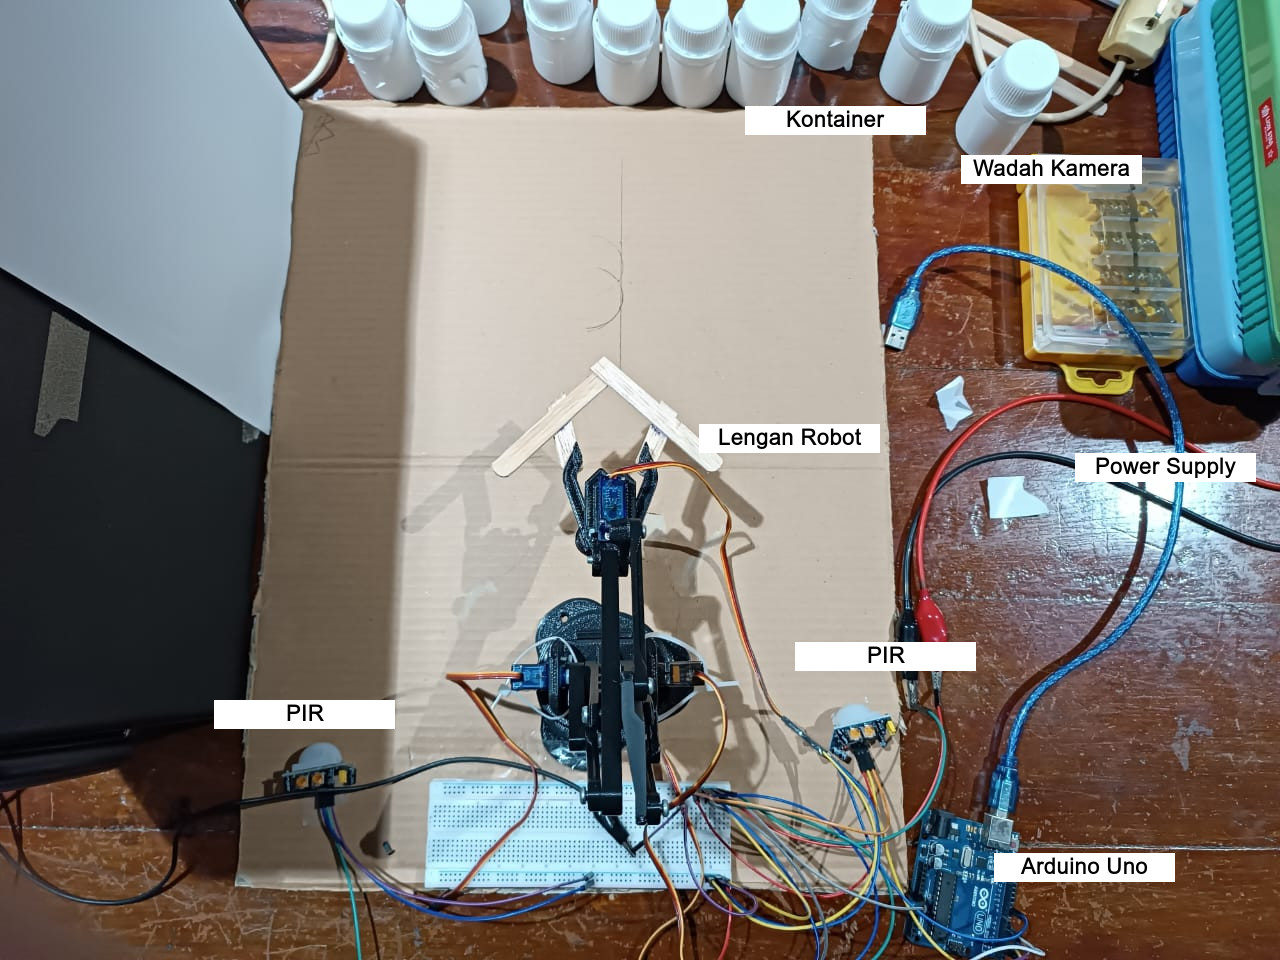
\includegraphics[width=0.7\textwidth]{gambar/rancang_sistem.jpg}
  \caption{Hasil perancangan sistem}
  \label{fig:rancang-sistem}
\end{figure}
\vspace{-1em}

\vspace{1em}

\section{Hasil Perancangan Model YOLO}
\subsection{Dataset dan \textit{Preprocessing}}
Tahap awal dalam penelitian ini adalah pengumpulan data primer berupa
citra kontainer menggunakan kamera. Proses akuisisi data dilakukan
untuk membangun sebuah dataset kustom yang merepresentasikan objek
target secara akurat. Total gambar mentah yang berhasil dikumpulkan
adalah 463 citra. Pengambilan gambar dilakukan dengan melakukan
variasi terhadap lokasi kontainer untuk memastikan model yang akan
dilatih nantinya mampu mengenali objek dengan baik. Dataset kemudian
dibagi menjadi 395 gambar untuk dataset latih dan 68 dataset
validasi. Distribusi pembagian dataset disajikan pada Tabel
\ref{tab:pembagian-dataset}.

\begin{table}[H]
  \caption{Distribusi pembagian dataset}
  \label{tab:pembagian-dataset}
  \vspace{-1em}
  \centering
  \begin{tabular}{ccc}
    \toprule
    \textbf{Kategori} & \textbf{Jumlah Gambar} & \textbf{Persentase} \\
    \midrule
    Data Latih & 395 & 85,3\% \\
    Data Validasi & 68 & 14,7\% \\
    Total Data & 463 & 100\% \\
    \bottomrule
  \end{tabular}
\end{table}

Setelah tahap akuisisi data, proses selanjutnya adalah anotasi
gambar. Anotasi merupakan proses fundamental untuk menghasilkan
dataset berlabel (\textit{labeled dataset}) yang akan digunakan
sebagai data pelatihan (\textit{training data}) \citep{19}. Dalam
konteks penelitian
ini, anotasi dilakukan dengan memberikan \textit{bounding box} serta label
kelas pada setiap objek di dalam gambar. Metode ini sangat penting
karena arsitektur YOLO dirancang untuk memprediksi \textit{bounding box} dan
probabilitas kelas secara bersamaan, sehingga memerlukan data latih
dengan format spesifik tersebut untuk dapat melakukan deteksi objek
secara \textit{real-time} \citep{20}. Sebanyak 463 gambar kontainer
telah dianotasi
secara manual. Contoh hasil anotasi dapat dilihat pada Gambar
\ref{fig:yolo-anotasi}.

\begin{figure}[H]
  \centering
  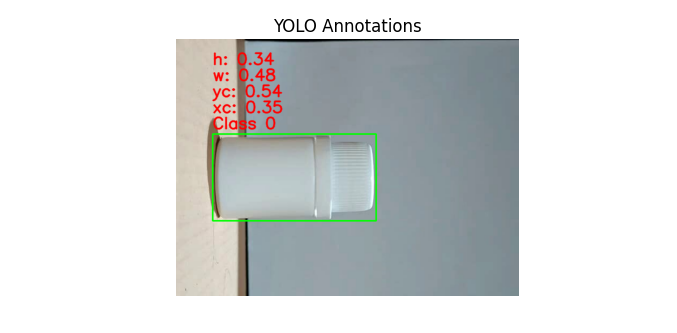
\includegraphics[width=1\textwidth]{gambar/anotasi.png}
  \caption{Salah satu data \textit{train} dengan labelnya}
  \label{fig:yolo-anotasi}
\end{figure}
\vspace{-1em}

\vspace{1em}

\subsection{Hasil Pelatihan Model}
Pada penelitian ini, \textit{mean Average Precision} (mAP) digunakan sebagai
metrik utama untuk mengukur performa model YOLO dalam mendeteksi
kontainer kimia. Akurasi deteksi ini sangat penting agar lengan robot
dapat melakukan inspeksi kecacatan secara tepat. Metrik ini dihitung
berdasarkan \textit{Average Precision} (AP), yang merupakan kombinasi dari
\textit{precision} dan \textit{recall} untuk setiap kelas secara
individual. Nilai mAP
sendiri adalah rata-rata AP untuk semua kelas, sehingga mampu
memberikan gambaran performa model yang komprehensif \citep{21}. \par

Untuk menentukan apakah sebuah prediksi dianggap benar (\textit{True
Positive}) atau salah (\textit{False Positive}), digunakanlah metrik
\textit{Intersection over Union} (IoU). IoU merupakan rasio antara area
tumpang tindih (\textit{overlap}) dari \textit{bounding box} hasil prediksi
($BB_{predict}$) dengan
\textit{bounding box ground truth} ($BB_{ground}$), dengan nilai berkisar antara
0 hingga 1 \citep{22}.
Semakin mendekati 1, berarti prediksi semakin akurat dan sesuai
dengan objek sebenarnya. IoU dihitung menggunakan persamaan:

\begin{equation}
  IoU = \frac{|BB_{predict} \cap
  BB_{ground}|}{|BB_{predict} \cup BB_{ground}|}
\end{equation}

\textit{Precision} mengukur proporsi prediksi positif yang benar (\textit{True
Positive}) terhadap seluruh prediksi positif (TP + \textit{False Positive}),
sehingga menunjukkan kemampuan model dalam meminimalkan kesalahan
deteksi. Sementara itu, \textit{recall} atau \textit{true positive
rate} mengukur seberapa banyak \textit{instance} positif sebenarnya yang
berhasil dideteksi dengan benar, sehingga menggambarkan kemampuan
model dalam menemukan semua objek yang ada \citep{23}. \textit{Precision} dan
\textit{recall} dapat dihitung menggunakan persamaan:

\begin{equation}
  Precision = \frac{TP}{TP + FP}, \quad
  Recall = \frac{TP}{TP + FN}
\end{equation}

mAP adalah nilai rata-rata dari AP untuk semua kelas. Karena model
YOLO yang digunakan dalam penelitian ini hanya
memprediksi satu kelas yaitu kontainer kimia, maka nilai mAP setara
dengan nilai AP. Nilai AP sendiri dihitung sebagai rata-rata
\textit{precision} di seluruh
rentang nilai \textit{recall} (0 hingga 1) \citep{24}, sebagaimana
dirumuskan dalam
Persamaan 3, di mana P adalah \textit{precision} dan r adalah \textit{recall}.

\begin{equation}
  AP = \int_{0}^{1} P(r) \,dr
\end{equation}

Proses pelatihan model YOLO dilakukan menggunakan \textit{platform}
\textit{Google
Colaboratory}. Model dilatih secara iteratif selama 50 \textit{epoch} dengan
\textit{batch size} 16 dan \textit{optimizer} Adam, agar model dapat mempelajari
fitur-fitur dari data latih secara optimal. Hasil pelatihan model
YOLO setiap 10 \textit{epoch} dapat dilihat pada Tabel \ref{tab:yolo-train}.

\begin{table}[H]
  \caption{Proses training model YOLO}
  \label{tab:yolo-train}
  \vspace{-1em}
  \centering
  \footnotesize
  \begin{tabular}{c p{1.5cm} p{1.5cm} p{1.5cm} p{1.5cm} p{1.5cm} p{1.5cm}}
    \toprule
    \textbf{Epoch} & \textbf{Train/Box Loss} & \textbf{Train/Class Loss}
    & \textbf{Train/DFL Loss} & \textbf{Val/Box Loss}
    & \textbf{Val/Class Loss} & \textbf{Val/DFL Loss} \\
    \midrule
    0 & 0.59460 & 1.93744 & 0.97064 & 0.47086 & 2.50286 & 0.89899 \\
    10 & 0.43332 & 0.43561 & 0.87133 & 0.30517 & 0.37575 & 0.82624 \\
    20 & 0.32857 & 0.29349 & 0.85098 & 0.33417 & 0.21048 & 0.84483 \\
    30 & 0.28212 & 0.23284 & 0.83904 & 0.24181 & 0.15662 & 0.82436 \\
    40 & 0.22672 & 0.17762 & 0.80096 & 0.22091 & 0.13860 & 0.82009 \\
    50 & 0.20164 & 0.15458 & 0.79927 & 0.20030 & 0.11625 & 0.81561 \\
    \bottomrule
  \end{tabular}
  \normalsize
\end{table}

Pada proses \textit{training}, nilai \textit{loss} pada data
\textit{train} dan validasi secara
umum menunjukkan tren penurunan seiring bertambahnya \textit{epoch}. Penurunan
ini menunjukkan bahwa model semakin mampu menyesuaikan parameter
internalnya dengan data yang diberikan. Dengan demikian, model
menjadi lebih baik dalam mempelajari pola yang relevan untuk
mendeteksi kontaier.

Pada \textit{Train/Box Loss}, terjadi penurunan signifikan dari 0.59460 pada
\textit{epoch} ke-0 menjadi 0.20164 pada \textit{epoch} ke-50, yang
mengindikasikan
peningkatan kemampuan model dalam memprediksi posisi \textit{bounding box}
secara lebih akurat. Hal serupa juga terlihat pada \textit{Train/Class Loss},
yang turun drastis dari 1.93744 menjadi 0.15458, menandakan model
semakin tepat dalam melakukan klasifikasi objek. Sementara itu,
\textit{Train/DFL Loss (Distribution Focal Loss)} menurun dari 0.97064 menjadi
0.79927, yang berarti model semakin baik dalam memperbaiki distribusi
prediksi \textit{bounding box}. Pada data validasi, \textit{Val/Box
Loss} menurun dari
0.47086 ke 0.20030, \textit{Val/Class Loss} dari 2.50286 ke 0.11625, serta
\textit{Val/DFL Loss} dari 0.89899 ke 0.81561. Penurunan yang konsisten pada
semua komponen \textit{loss} validasi menunjukkan bahwa model tidak hanya
mampu belajar dengan baik pada data \textit{train}, tetapi juga memiliki
kemampuan generalisasi yang baik terhadap data yang belum pernah
dilihat sebelumnya.

Namun, evaluasi kinerja model tidak bisa hanya mengandalkan nilai
loss. Perlu digunakan metrik tambahan seperti mAP  untuk menilai
akurasi deteksi dan kualitas prediksi \textit{bounding box} secarah
menyeluruh. Pada penelitian ini digunakan mAP@50 (IoU \textit{threshold} 50\%)
untuk mengukur keberhasilan deteksi secara lebih longgar, serta
mAP@95 (rata-rata mAP dari IoU \textit{threshold} 50\% hingga 95\% dengan
interval 5\%) untuk menilai ketepatan prediksi \textit{bounding box} secara
lebih ketat dan detail. Hasil pengukuran mAP pada tiap \textit{epoch} dapat
dilihat pada Gambar \ref{fig:map}.

\begin{figure}[H]
  \centering
  % First image
  \begin{minipage}[t]{0.48\textwidth}
    \centering
    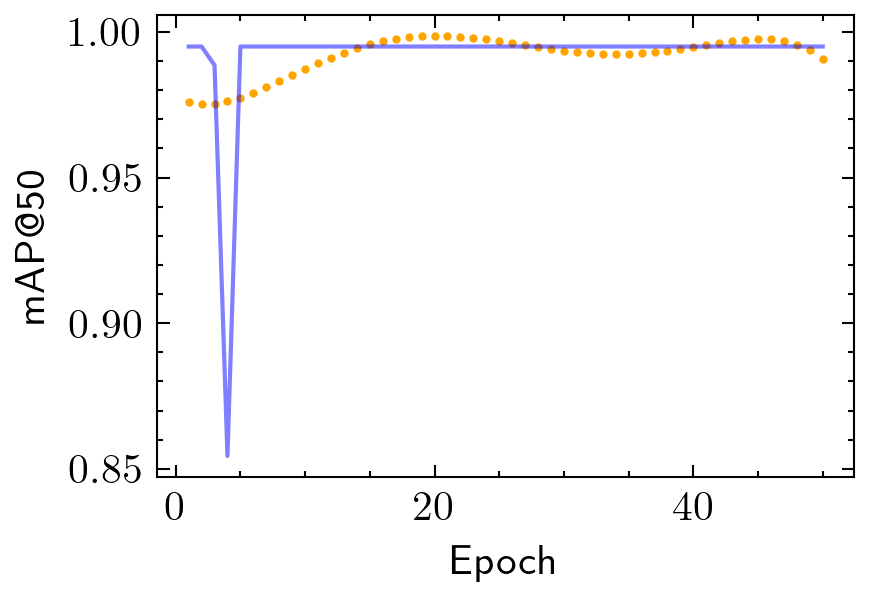
\includegraphics[width=\textwidth]{gambar/map50.png}
    (a)
  \end{minipage}
  \hfill
  % Second image
  \begin{minipage}[t]{0.48\textwidth}
    \centering
    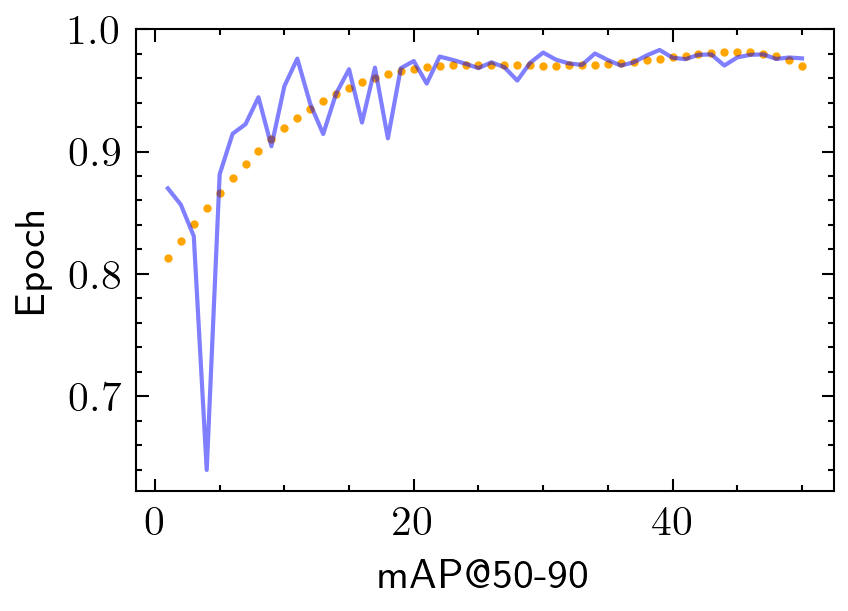
\includegraphics[width=\textwidth]{gambar/map5090.png}
    (b)
  \end{minipage}
  \caption{Grafik tren mAP: (a) mAP@50, (b) mAP@50-90}
  \label{fig:map}
  \vspace{-1em}
\end{figure}

Grafik tersebut menyajikan evaluasi performa model deteksi objek
menggunakan metrik mAP seiring berjalannya
50 \textit{epoch} pelatihan. Grafik di sebelah kiri, mAP@50, yang menggunakan
ambang batas IoU longgar (50\%), menunjukkan bahwa model dengan
sangat cepat mencapai performa puncak. Terlihat bahwa nilainya
melonjak mendekati 1.00 hanya dalam 10-15 \textit{epoch} pertama lalu
cenderung datar, menandakan model mampu mempelajari cara mendeteksi
keberadaan objek secara umum dengan sangat cepat. Sebaliknya, grafik
di sebelah kanan, mAP@50-95, yang mengukur performa pada rentang
ambang batas IoU yang lebih ketat (50\% hingga 95\%), menunjukkan
kurva pembelajaran yang lebih bertahap dan konsisten. Peningkatan
yang lebih landai ini mengindikasikan bahwa model menggunakan
mayoritas waktu pelatihannya untuk terus-menerus menyempurnakan
presisi dan akurasi lokalisasi bounding box-nya. Secara keseluruhan,
pencapaian nilai mAP yang sangat tinggi pada kedua metrik di akhir
pelatihan menandakan model final yang dihasilkan tidak hanya mampu
mendeteksi objek, tetapi juga sangat akurat dalam menentukan
batas-batasnya. Hasil deteksi kontainer kimia pada data validasi
dapat dilihat pada Gambar \ref{fig:yolo-validasi}.

\begin{figure}[H]
  \centering
  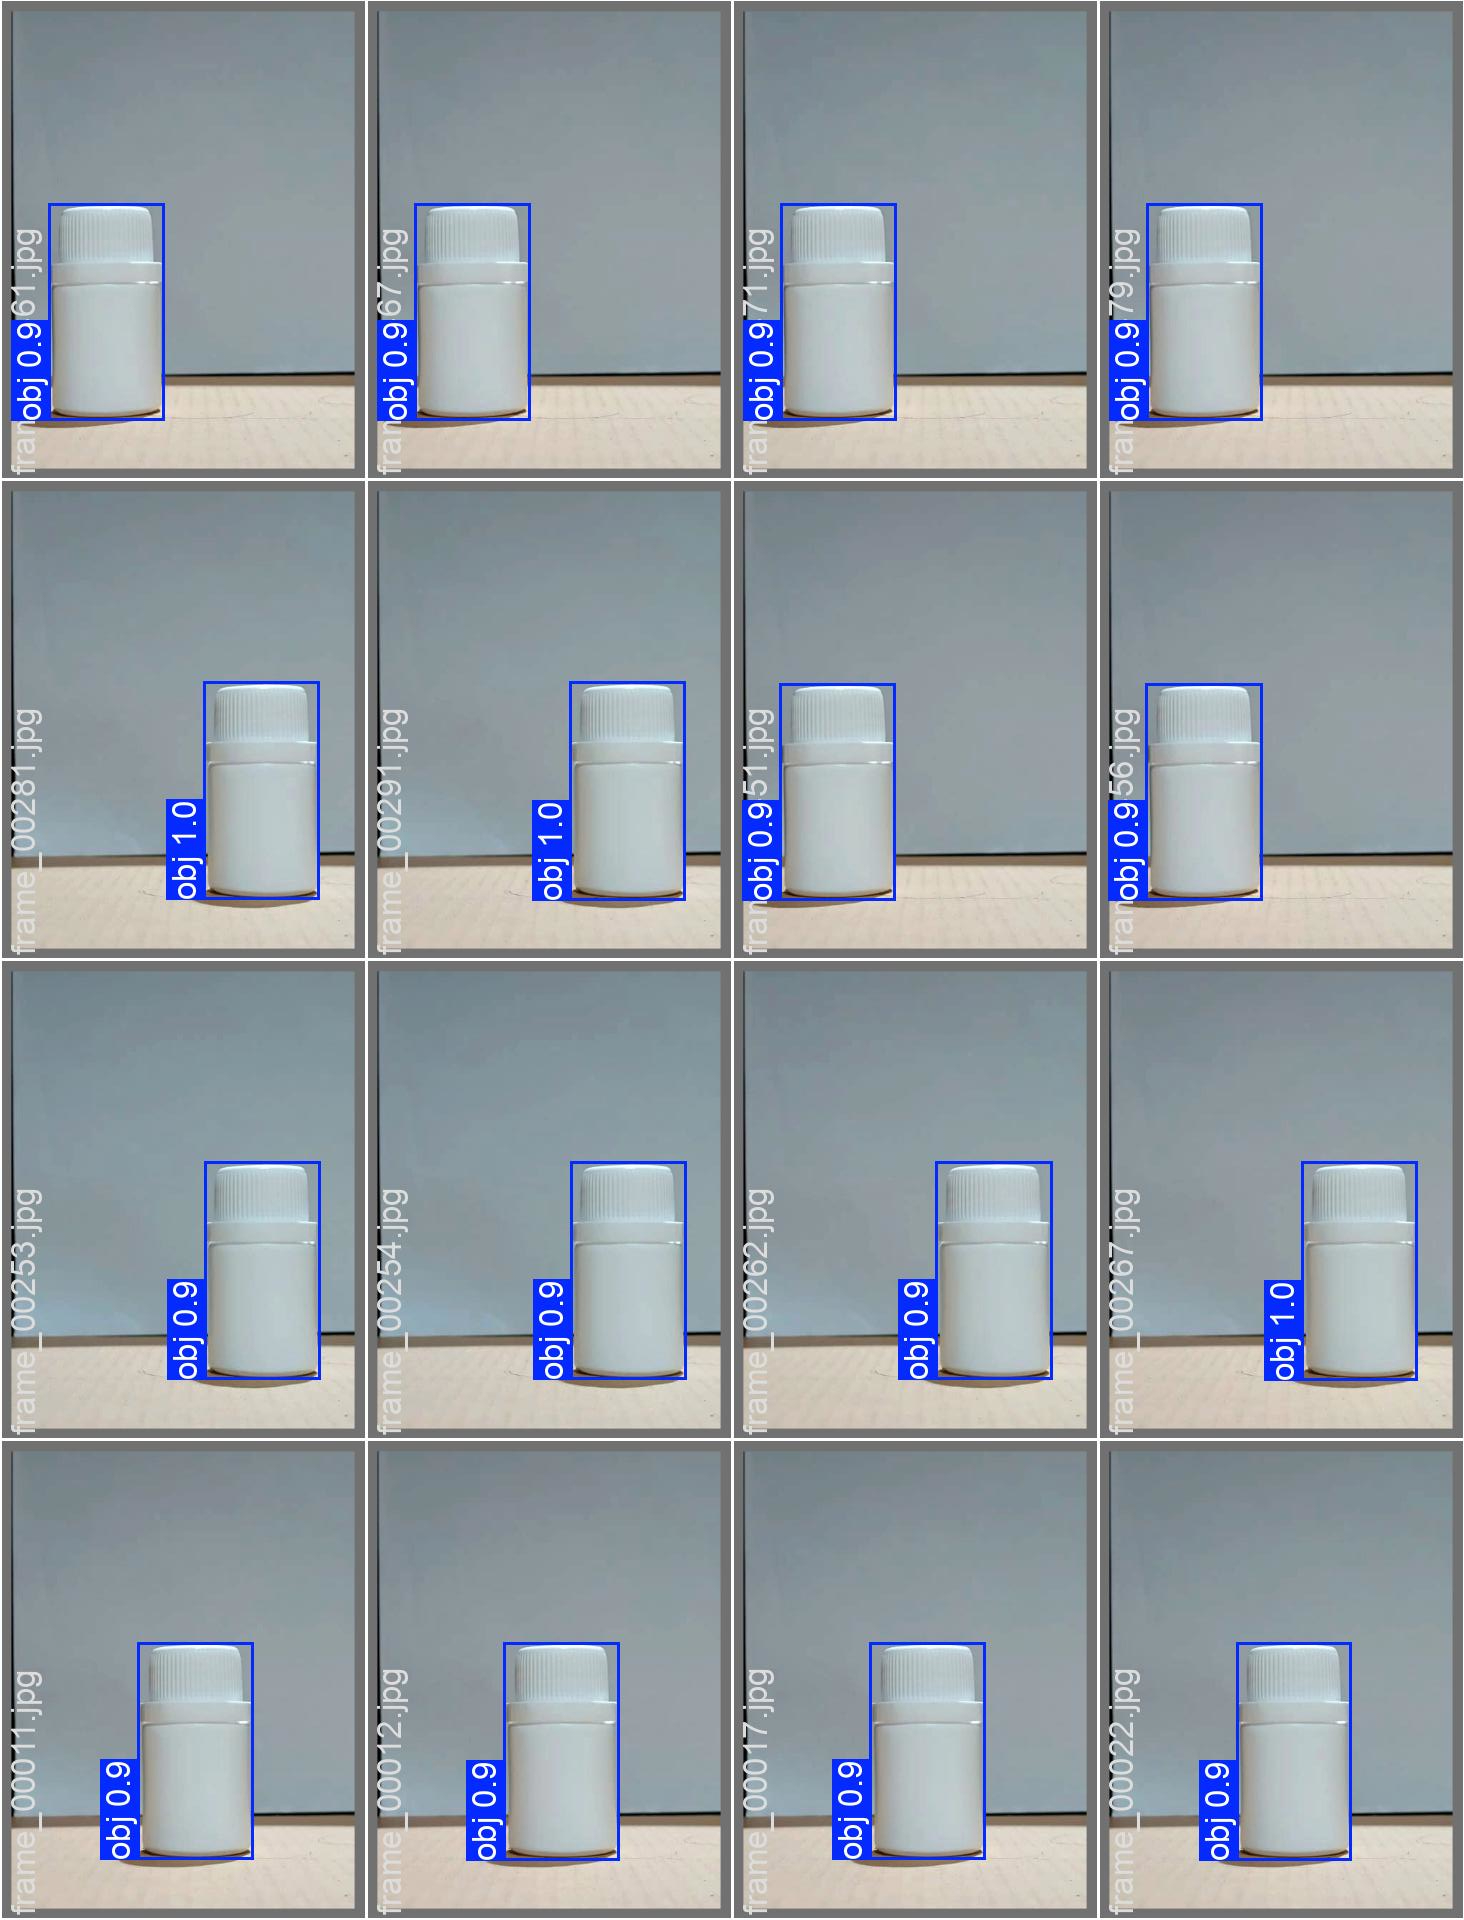
\includegraphics[width=0.7\textwidth]{gambar/yolo_validasi.jpg}
  \caption{Hasil prediksi YOLO pada data validasi}
  \label{fig:yolo-validasi}
\end{figure}
\vspace{-1em}

\vspace{1em}

\section{Hasil Perancangan Model Deteksi Kecacatan}
\subsection{Arsitektur Variational Autoencoder}
\textit{Variational autoencoder} (VAE) merupakan pengembangan dari
\textit{autoencoder}, yaitu sebuah arsitektur \textit{neural network}
yang berfungsi untuk mengekstrak fitur laten dari data. Perbedaan
fundamental VAE dibandingkan pendahulunya terletak pada pendekatan
Bayesian, di mana vektor laten ($z$) dipaksa mengikuti distribusi
probabilitas terstruktur, umumnya distribusi Gaussian. Secara
operasional, encoder VAE ($q_{\phi}(z \mid x)$) tidak hanya
mengompres data \textit{input} ($x$), melainkan juga memetakannya
ke dalam parameter statistik: sebuah vektor mean (rata-rata) dan
vektor varians. Selanjutnya, sebuah sampel kode laten ($z$) diambil
dari distribusi yang diwakili oleh kedua parameter ini, lalu diumpankan
ke decoder ($p_{\theta}(x \mid z)$) untuk merekonstruksi data \textit{input}
asli \citep{25}. Arsitektur variational autoencoder yang digunakan pada
penelitian ini dapat dilihat pada Gambar x.

Arsitektur VAE yang diimplementasikan pada penelitian ini dirancang
untuk memproses citra berukuran 128 $\times$ 128 dengan tiga kanal
warna (RGB). Bagian \textit{encoder} menggunakan lima lapis
\textit{convolutional} berurutan, masing-masing diikuti fungsi
aktivasi ReLU, untuk secara progresif mengekstrak dan menurunkan
resolusi fitur spasial, hingga menghasilkan representasi akhir
berukuran (512, 4, 4). Representasi ini kemudian diproyeksikan
menjadi dua vektor, yaitu vektor
\textit{mean} dan vektor \textit{log-varians}, yang mendefinisikan
distribusi Gaussian
multivariat sebagai ruang laten. Setelah sampling vektor laten $z$,
\textit{decoder} memproyeksikan kembali $z$ ke dimensi spasial melalui lapisan
linear dan serangkaian lapisan \textit{transpose convolutional}
(dekonvolusi) yang secara bertahap memperbesar resolusi hingga
kembali ke ukuran asli citra \textit{input}. Fungsi aktivasi sigmoid pada
lapisan output memastikan nilai piksel berada pada rentang $[0, 1]$,
sehingga hasil rekonstruksi dapat diinterpretasikan sebagai citra valid.

\vspace{1em}

\subsection{Dataset dan \textit{Preprocessing}}
Tahap ini adalah pengumpulan data primer berupa
citra kontainer menggunakan kamera. Proses akuisisi data ini
dilakukan untuk membangun dataset kustom yang secara spesifik
merepresentasikan objek target. Total gambar mentah yang berhasil
dikumpulkan berjumlah 3000 citra, yang seluruhnya digunakan sebagai
dataset latih. Sebelum digunakan untuk pelatihan autoencoder, seluruh
citra diproses menggunakan model YOLO untuk mendeteksi serta
melakukan \textit{cropping} area kontainer
secara otomatis. Dengan demikian, hanya bagian kontainer yang relevan
yang masuk ke pipeline pemrosesan, sehingga model autoencoder dapat
lebih fokus dalam mempelajari fitur visual kontainer secara mendalam.
Contoh salah satu data dapat dilihat pada Gambar x.

Karena \textit{autoencoder} termasuk dalam kategori \textit{unsupervised
learning}, data yang digunakan pada penelitian ini tidak memerlukan
label atau anotasi manual. Seluruh dataset hanya terdiri dari citra
kontainer yang dalam kondisi baik (bebas kerusakan atau cacat
visual), sehingga model \textit{autoencoder} dapat belajar merepresentasikan
distribusi citra kontainer normal secara optimal. Dengan demikian,
\textit{autoencoder} akan berfokus pada rekonstruksi citra input semirip
mungkin, dan nantinya dapat digunakan untuk mendeteksi anomali atau
kerusakan berdasarkan perbedaan signifikan antara citra asli dan
hasil rekonstruksi.

\vspace{1em}

\subsection{Hasil Pelatihan Model}

Fungsi \textit{loss} VAE didasarkan pada \textit{Evidence Lower
Bound} (ELBO). Tujuannya
adalah memaksimalkan \textit{bound} ini agar dapat mengatasi masalah
distribusi posterior yang tidak dapat dihitung secara langsung pada
model probabilistik. Fungsi \textit{loss} terdiri dari dua komponen utama.
Komponen pertama adalah \textit{reconstruction loss}, yang merupakan
ekspektasi dari error rekonstruksi negatif. Komponen ini mengukur
seberapa baik \textit{decoder} probabilistik, $p_\theta(x|z)$, dapat
merekonstruksi data \textit{input} $x$ dari representasi laten $z$. Komponen
kedua adalah \textit{regularization term}, yang dihitung sebagai
Kullback-Leibler (KL) \textit{divergence} antara distribusi posterior
aproksimasi $q_\phi(z|x)$ dan distribusi prior $p_\theta(z)$.
Komponen ini berfungsi sebagai penalti, supaya distribusi yang
dihasilkan encoder tetap mendekati distribusi prior sederhana
seperti distribusi Gaussian \citep{26}. Secara matematis, fungsi \textit{loss}
VAE dapat ditulis sebagai:

\begin{equation}
  \mathcal{L}(\theta, \phi; x) = \mathbb{E}{q\phi(z|x)}[\log
  p_\theta(x|z)] - D_{KL}(q_\phi(z|x) \parallel p_\theta(z))
\end{equation}

Proses pelatihan model \textit{variational autoencoder} dilakukan
menggunakan platform Google
Colaboratory. Model dilatih secara iteratif selama 100 epoch dengan
\textit{batch size} 64
dan \textit{optimizer} Adam, agar model dapat mempelajari fitur-fitur dari
data latih secara
optimal. Hasil pelatihan model YOLO setiap 10 epoch dapat dilihat
pada Tabel \ref{tab:training-autoencoder}.

\begin{table}[H]
  \caption{Distribusi pembagian dataset}
  \label{tab:training-autoencoder}
  \vspace{-1em}
  \centering
  \begin{tabular}{cc}
    \toprule
    \textbf{Epoch} & \textbf{Loss} \\
    \midrule
    1 & 837.7615 \\
    10 & 30.5440 \\
    20 & 22.6941 \\
    30 & 18.5220 \\
    40 & 15.0172 \\
    50 & 11.9098 \\
    60 & 9.8593 \\
    70 & 8.7772 \\
    80 & 7.3923 \\
    90 & 7.1070 \\
    100 & 6.8338 \\
    \bottomrule
  \end{tabular}
\end{table}

Pada proses \textit{training}, nilai \textit{loss} rekonstruksi
secara umum menunjukkan tren penurunan seiring bertambahnya
\textit{epoch}. Penurunan ini mengindikasikan bahwa model autoencoder
semakin mampu mempelajari representasi fitur penting dari data normal
yang diberikan. Dengan demikian, model menjadi lebih baik dalam
merekonstruksi kontainer kimia tanpa cacat, sehingga mempermudah
deteksi perbedaan (anomali) ketika diaplikasikan pada data cacat.
Hasil prediksi kecacatan \textit{training} dapat dilihat
pada Gambar \ref{fig:autoencoder-test}.

\begin{figure}[H]
  \centering
  % First image
  \begin{minipage}{0.8\textwidth}
    \centering
    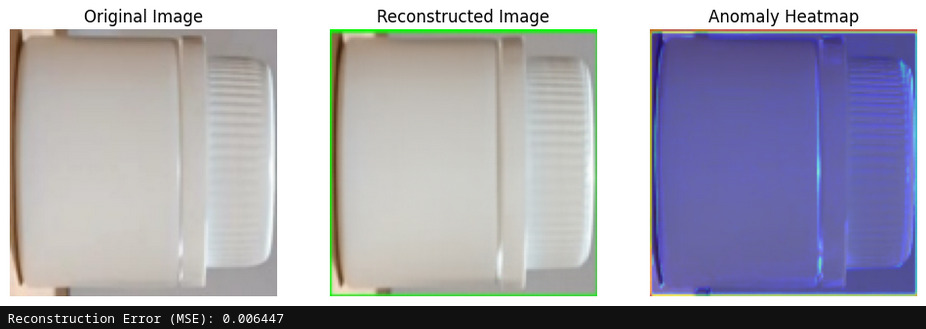
\includegraphics[width=\textwidth]{gambar/kontainer_bagus.jpeg}
    (a)
  \end{minipage}
  \vspace{1em}

  % Second image
  \begin{minipage}{0.8\textwidth}
    \centering
    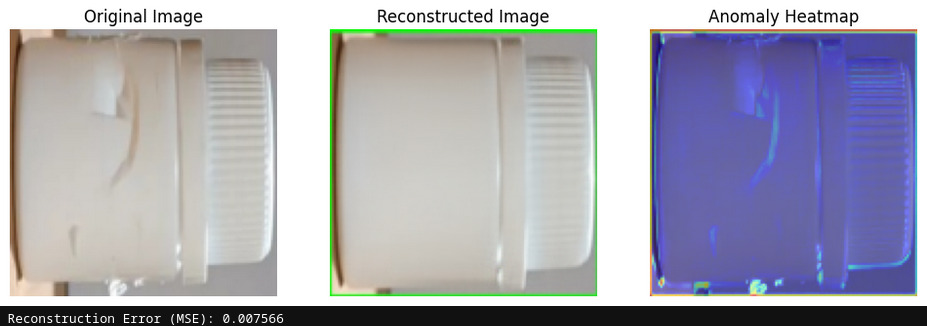
\includegraphics[width=\textwidth]{gambar/kontainer_cacat.jpeg}
    (b)
  \end{minipage}
  \caption{Hasil prediksi kecacatan: (a) Kontainer normal, (b) kontainer cacat}
  \label{fig:autoencoder-test}
  \vspace{-1em}
\end{figure}

Gambar di atas menunjukkan rekonstruksi \textit{error} model
\textit{autoencoder} pada kontainer normal dan cacat. Pada kontainer
normal, \textit{error} yang diperoleh adalah 0.006447 sedangkan pada
kontainer cacat sebesar 0.007566. Dari hasil tersebut terlihat
\textit{error} pada kontainer cacat lebih besar dibandingkan
\textit{error} pada kontainer normal. Hal ini menunjukkan bahwa model
sudah dapat membedakan kontainer normal dan cacat.

\vspace{1em}

\subsection{Penentuan Threshold Kecacatan}
Penentuan threshold sangat penting agar sistem deteksi cacat dapat
membedakan secara akurat antara kontainer kimia yang cacat dan yang
normal. Tanpa threshold yang tepat, model berpotensi menghasilkan
banyak kesalahan prediksi, sehingga mengurangi keandalan sistem.
Dalam penelitian
ini, metrik \textit{error} yang digunakan untuk mengukur perbedaan antara
citra asli dan hasil rekonstruksi adalah \textit{Mean Squared Error} (MSE).

MSE merupakan metrik yang paling umum digunakan untuk mengukur
kualitas citra secara kuantitatif. MSE menghitung rata-rata selisih
kuadrat antara piksel citra asli (\textit{input}) dengan piksel citra hasil
rekonstruksi (\textit{output}). Semakin kecil nilai MSE, semakin mirip citra
hasil rekonstruksi dengan citra aslinya, yang berarti model berhasil
meminimalkan distorsi \citep{27}. MSE dirumuskan sebagai berikut:

\begin{equation}
  MSE = \frac{1}{n} \sum_{i=1}^{n} (x_i - \hat{x}_i)^2
\end{equation}

Pengujian dilakukan pada 20 gambar kontainer kimia, terdiri dari 10
gambar kontainer normal dan 10 gambar kontainer cacat. Dari pengujian
ini diperoleh distribusi nilai MSE masing-masing gambar untuk
dianalisis lebih lanjut. Hasil perhitungan MSE pada 20 gambar uji
tersebut dirangkum pada \ref{tab:error-samples}.

\begin{table}[H]
  \centering
  \caption{Nilai error untuk setiap sampel}
  \label{tab:error-samples}
  \begin{tabular}{ccc}
    \toprule
    \textbf{Index} & \textbf{Error} & \textbf{Kategori} \\
    \midrule
    1  & 0.006737 & Normal \\
    2  & 0.006828 & Normal \\
    3  & 0.007091 & Normal \\
    4  & 0.006997 & Normal \\
    5  & 0.006610 & Normal \\
    6  & 0.006795 & Normal \\
    7  & 0.006872 & Normal \\
    8  & 0.006725 & Normal \\
    9  & 0.006873 & Normal \\
    10 & 0.006817 & Normal \\
    11 & 0.007432 & Cacat \\
    12 & 0.007455 & Cacat \\
    13 & 0.008369 & Cacat \\
    14 & 0.007183 & Cacat \\
    15 & 0.007653 & Cacat \\
    16 & 0.008856 & Cacat \\
    17 & 0.007531 & Cacat \\
    18 & 0.007624 & Cacat \\
    19 & 0.007457 & Cacat \\
    20 & 0.008424 & Cacat \\
    \bottomrule
  \end{tabular}
\end{table}

Tabel \ref{tab:error-samples} menunjukkan nilai \textit{error} atau selisih
rekonstruksi (dihitung menggunakan MSE) pada masing-masing sampel
gambar, yang terdiri dari 10 kontainer normal dan 10 kontainer cacat.
Terlihat bahwa sampel dengan kategori normal memiliki nilai error
yang relatif kecil dan cukup seragam di sekitar 0.0067, menandakan
model mampu merekonstruksi dengan baik. Sebaliknya, sampel dengan
kategori cacat cenderung memiliki error lebih tinggi, menunjukkan
adanya perbedaan yang signifikan pada area cacat yang gagal
direkonstruksi dengan sempurna, sehingga mempermudah deteksi anomali.

Kurva \textit{Receiver Operating Characteristic} (ROC) digunakan
sebagai metode analisis untuk mengevaluasi performa model deteksi
cacat pada kontainer kimia dalam penelitian ini. Kurva ROC dibuat
dengan memplot nilai 1 - \textit{precision} (\textit{false positive
rate}) pada sumbu
x dan \textit{recall} (\textit{true positive rate}) pada sumbu y untuk setiap
nilai ambang (\textit{threshold}) yang diuji. Nilai
\textit{threshold} terbaiki ditentukan dengan memaksimalkan statistik
Youden J \citep{28}. Kurva ROC dapat dilihat pada Gambar
\ref{fig:roc}. Persamaan
statistik Youden J dituliskan sebagai berikut:
\begin{equation}
  J = \textit{Recall} + \textit{Precision} - 1
\end{equation}

\begin{figure}[H]
  \centering
  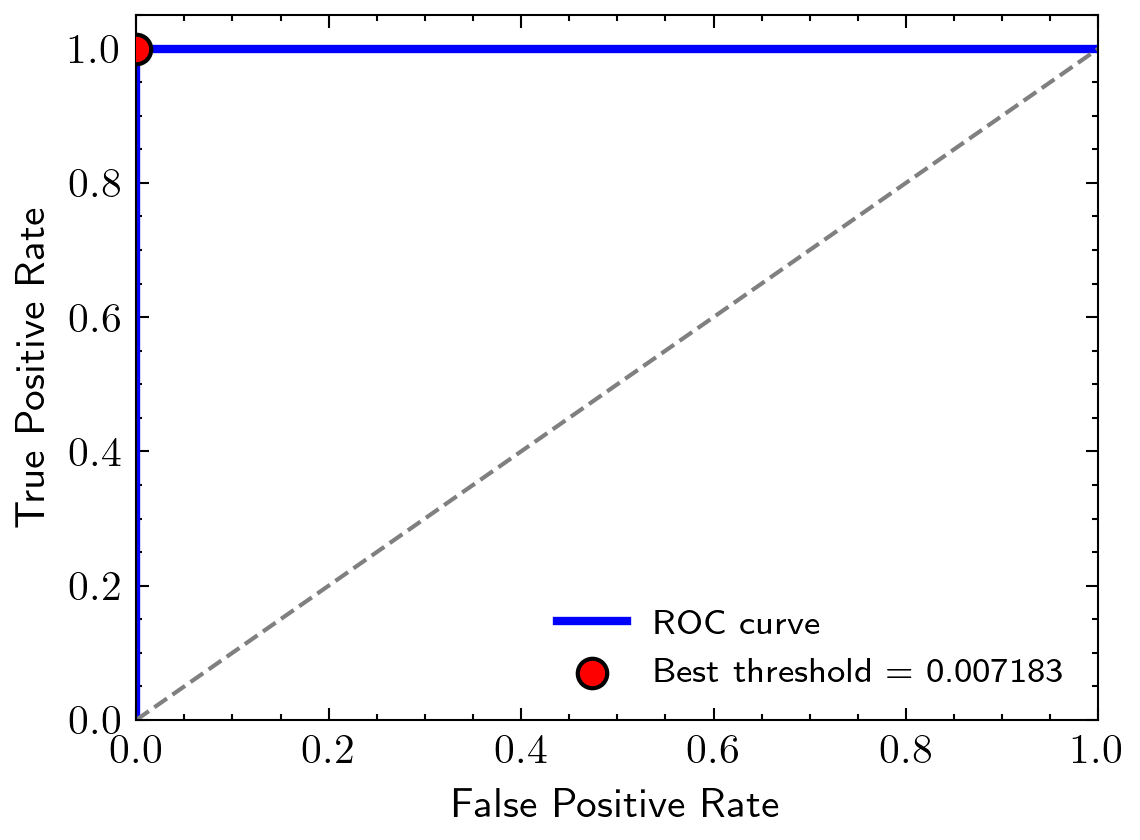
\includegraphics[]{gambar/roc.png}
  \caption{Kurva ROC}
  \label{fig:roc}
\end{figure}
\vspace{-1em}

Kurva di atas menunjukkan performa model dalam membedakan kontainer
cacat dan tidak cacat dengan sangat baik, ditunjukkan oleh garis biru
yang mendekati titik sudut kiri atas. Berdasarkan perhitungan,
threshold optimal yang diperoleh adalah sebesar 0.007183, ditandai
dengan lingkaran merah pada grafik. Nilai ini digunakan sebagai batas
deteksi akhir, sehingga model dapat memaksimalkan sensitivitas
sekaligus meminimalkan kesalahan positif dalam identifikasi cacat.

\vspace{1em}

\section{Hasil Pengujian Sistem Lengan Robot}

Setelah model deteksi terlatih dan nilai threshold optimal
ditentukan, tahap selanjutnya adalah integrasi sistem dengan lengan
robot yang dikontrol oleh mikrokontroler Arduino. Berdasarkan hasil
klasifikasi dari model, lengan robot akan secara otomatis memindahkan
kontainer kimia. Objek akan diarahkan ke sebelah kiri jika sistem
mengidentifikasinya sebagai cacat, dan ke sebelah kanan jika
dinyatakan normal. Gambar \ref{fig:robot-only} mengilustrasikan aksi lengan
robot ketika sedang menyortir objek yang teridentifikasi cacat.

\begin{figure}[H]
  \centering
  % First image
  \begin{minipage}[t]{0.48\textwidth}
    \centering
    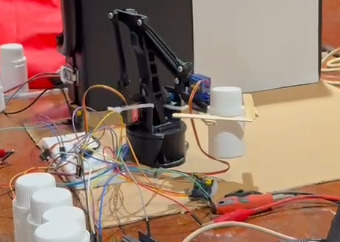
\includegraphics[width=\textwidth]{gambar/robot_normal.jpeg}
    (a)
  \end{minipage}
  \hfill
  % Second image
  \begin{minipage}[t]{0.48\textwidth}
    \centering
    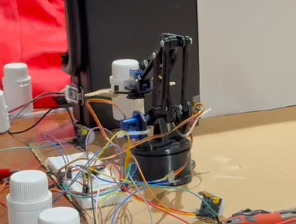
\includegraphics[width=\textwidth]{gambar/robot_cacat.jpeg}
    (b)
  \end{minipage}
  \caption{Lengan robot menyortir kontainer: (a) normal, (b) cacat}
  \label{fig:robot-only}
  \vspace{-1em}
\end{figure}

Setelah lengan robot melepaskan kontainer di area penyortiran yang
telah ditentukan (kiri untuk cacat, kanan untuk normal), sebuah
sensor PIR yang terpasang di lokasi tersebut akan
mendeteksi keberadaan objek. Deteksi dari sensor PIR ini berfungsi
sebagai sinyal konfirmasi bahwa satu siklus penyortiran telah
selesai. Sinyal ini kemudian memicu pengiriman data hasil
klasifikasi, yang mencakup citra kontainer beserta label statusnya,
ke server pusat. Untuk menampilkan informasi ini secara dinamis dan
instan kepada klien, sistem memanfaatkan protokol \textit{WebSocket}.
Tampilan website dan hasil prediksi dapat dilihat pada Gambar
\ref{fig:web-test}.

\begin{figure}[H]
  \centering
  % First image
  \begin{minipage}{0.8\textwidth}
    \centering
    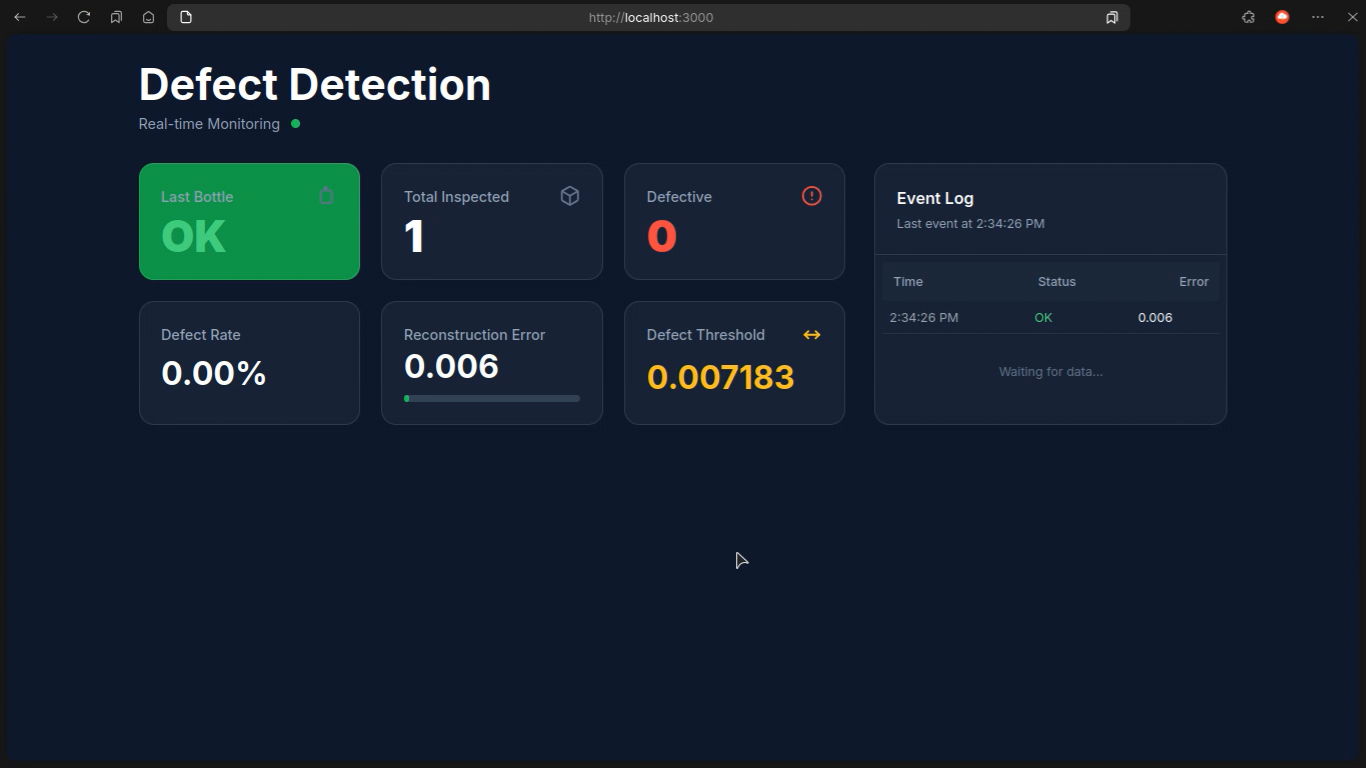
\includegraphics[width=\textwidth]{gambar/web_ss_normal.png}
    (a)
  \end{minipage}
  \vspace{1em}

  % Second image
  \begin{minipage}{0.8\textwidth}
    \centering
    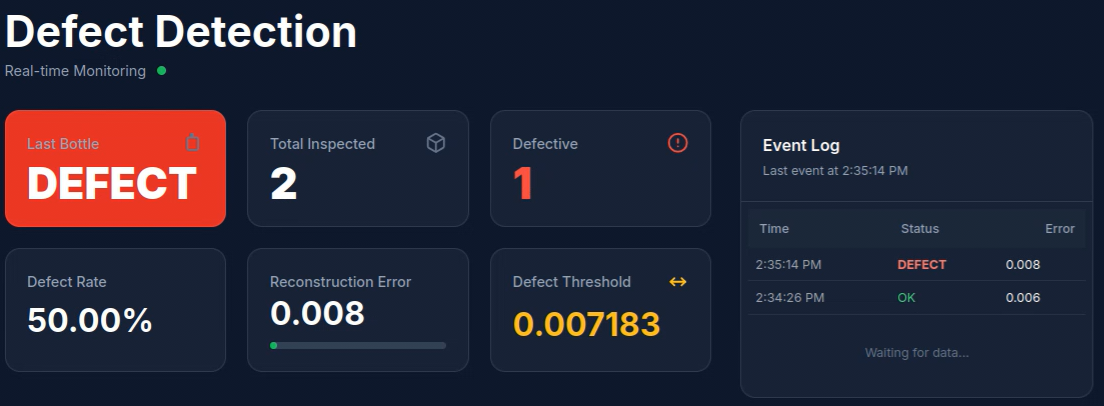
\includegraphics[width=\textwidth]{gambar/web_ss_cacat.png}
    (b)
  \end{minipage}
  \caption{Hasil prediksi website: (a) Kontainer normal, (b) kontainer cacat}
  \label{fig:web-test}
  \vspace{-1em}
\end{figure}

Untuk menguji keandalan dan konsistensi performa model, dilakukan
serangkaian pengujian sebanyak 25 kali pada objek kontainer. Setiap
pengujian menggunakan sampel dengan kondisi yang bervariasi antara
normal dan cacat untuk mengevaluasi kemampuan generalisasi model.
Hasil kuantitatif dari setiap pengujian ini dirangkum secara rinci
pada Tabel \ref{tab:error-samples-web}.

\begin{table}[H]
  \centering
  \caption{Nilai error untuk setiap sampel}
  \label{tab:error-samples-web}
  \begin{tabular}{cccc}
    \toprule
    \textbf{Index} & \textbf{Error} & \textbf{Kategori (Threshold <
    0.007183)} & \textbf{Label Asli} \\
    \midrule
    1  & 0.006798 & Normal & Normal \\
    2  & 0.008298 & Cacat & Cacat \\
    3  & 0.006854 & Normal & Normal \\
    4  & 0.007066 & Normal & Normal \\
    5  & 0.006923 & Normal & Normal \\
    6  & 0.007607 & Cacat & Cacat \\
    7  & 0.007261 & Cacat & Cacat \\
    8  & 0.007393 & Cacat & Cacat \\
    9  & 0.006842 & Normal & Normal \\
    10 & 0.008099 & Cacat & Cacat \\
    11 & 0.006945 & Normal & Normal \\
    12 & 0.007381 & Cacat & Cacat \\
    13 & 0.006722 & Normal & Normal \\
    14 & 0.006865 & Normal & Normal \\
    15 & 0.007397 & Cacat & Cacat \\
    16 & 0.007099 & Normal & Normal \\
    17 & 0.006790 & Normal & Normal \\
    18 & 0.006760 & Normal & Normal \\
    19 & 0.007383 & Cacat & Cacat \\
    20 & 0.007693 & Cacat & Cacat \\
    21 & 0.008071 & Cacat & Cacat \\
    22 & 0.007977 & Cacat & Cacat \\
    23 & 0.006885 & Normal & Normal \\
    24 & 0.008007 & Cacat & Cacat \\
    25 & 0.006847 & Normal & Normal \\
    \midrule
    \multicolumn{3}{r}{\textbf{Tingkat Akurasi}} & \textbf{100\%} \\
    \bottomrule
  \end{tabular}
\end{table}

Tabel \ref{tab:error-samples-web} menyajikan hasil pengujian
performa model deteksi kecacatan pada 25 sampel kontainer yang
berbeda untuk memvalidasi efektivitasnya. Keputusan klasifikasi untuk
setiap sampel didasarkan pada perbandingan nilai error rekonstruksi
terhadap ambang batas (threshold) yang telah ditentukan sebesar
0.007183. Sesuai dengan mekanisme ini, objek dengan nilai error di
bawah threshold dikategorikan sebagai "Normal", sementara objek
dengan nilai error yang melebihinya dikategorikan sebagai "Cacat".
Hasil pada tabel secara jelas menunjukkan bahwa untuk keseluruhan 25
data uji, kolom "Kategori" (label prediksi dari model) sepenuhnya
konsisten dengan kolom "Label Asli" (kondisi faktual objek). Sebagai
contoh, pada data indeks ke-2, nilai error yang tinggi (0.008298)
berhasil diidentifikasi dengan benar sebagai "Cacat", sementara pada
data indeks ke-1, nilai error yang rendah (0.006798) juga tepat
diklasifikasikan sebagai "Normal". Kesesuaian sempurna antara
prediksi dan kondisi sebenarnya pada seluruh rangkaian pengujian ini
membuktikan bahwa model, dengan threshold yang dipilih, mampu
mencapai tingkat akurasi 100\% dalam membedakan antara kontainer
normal dan cacat. Gambar \ref{fig:web-25} menampilkan hasil website
setelah melakukan prediksi terhadap 25 sampel.

\begin{figure}[H]
  \centering
  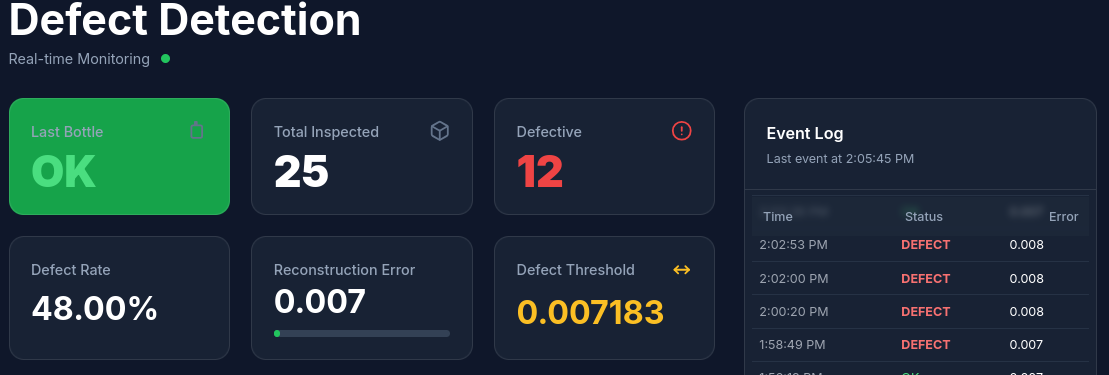
\includegraphics[width=0.7\textwidth]{gambar/ss_web_25.png}
  \caption{Hasil prediksi kecacatan pada 25 sampel}
  \label{fig:web-25}
\end{figure}
\vspace{-1em}
